% This LMU slides template is adapted from the beaver colortheme by Shengqiang Zhang.
\documentclass{beamer}

\usepackage[utf8]{inputenc}
\usepackage{natbib}
\usepackage{multirow}
\usepackage{booktabs}
\usepackage{float}
\usepackage{bbding}
\usepackage{array}
\usepackage{tikz}
\usetikzlibrary{automata, positioning, arrows}
\usepackage{amsmath}
\let\Tiny\tiny
\beamertemplatenavigationsymbolsempty

\usetheme{Madrid}
% \usetheme{Darmstadt}
% \usetheme{Rochester}
% \usetheme{Frankfurt}
% \usetheme{CambridgeUS}
% \usetheme{default}
% \usefonttheme{serif} %times new roman
\definecolor{Green}{RGB}{43,134,75}
\usecolortheme{lmugreen}
\setbeamercolor{item projected}{bg=Green,fg=white}
% \definecolor{UBCblue}{rgb}{0.04706, 0.13725, 0.26667} % UBC Blue (primary)

% \usecolortheme[named=LMUGreen]{structure}

\begin{document}
\title[Algebra \& Computer Science]{Formal languages and automatas}
\author[Ruben Triwari]{Ruben Triwari}
\institute[LMU Munich]{
    % \large
    {
\includegraphics[scale=0.032]{images/LMU_Muenchen_Logo.svg.png}} \\
    Seminar: Algebra \& Computer Science, LMU Munich 
}
\date{July 6, 2024}


% \titlegraphic{
%     \begin{tikzpicture}[remember picture,overlay]
%     \node[anchor=south east, yshift=8pt, xshift=0pt] at (current page.south east)
%     {
\includegraphics[scale=0.032]{images/LMU_Muenchen_Logo.svg.png}};
%     \end{tikzpicture}
% }

\addtobeamertemplate{frametitle}{}{%
\begin{tikzpicture}[remember picture,overlay]
\node[anchor=north east,yshift=8pt, xshift=7pt] at (current page.north east) {
\includegraphics[scale=0.022]{images/LMU_Muenchen_Logo.svg.png}};
\end{tikzpicture}
\vspace{-10pt}
}

\AtBeginSection[]
{
  \begin{frame}
    \frametitle{Outline}
    \tableofcontents[currentsection]
  \end{frame}
}
\frame{\titlepage}

\section{History \& Motivation}
\section{Formal Languages Definitions, Examples}
\begin{frame}
  \frametitle{Alphabets \& Languages}
  An Alphabet $\Sigma$ is a set of characters.\\
  Examples:
  \begin{enumerate}
    \item $\Sigma = \{a,b,c\}$
    \item $\Sigma = \{x\}$
    \item $\Sigma = \emptyset$
  \end{enumerate}
  A Language $L$ is a set of words with characters 
  out of an Alphabet $\Sigma$.\\
  Examples:
  \begin{enumerate}
    \item $\Sigma = \{a,b,c\} \rightsquigarrow L = \{aaa, bbb, ccc, abc\}$
    \item $\Sigma = \{x\} \rightsquigarrow L = \{ x, xx, xxx, xxxx\}$
    \item $\Sigma = \emptyset \rightsquigarrow L = \{\epsilon \}$
  \end{enumerate}
  $\rightsquigarrow L \subset \Sigma^*$
\end{frame}

\begin{frame}
  \frametitle{Formal series}
  We can also write a Language with a formal series, with a fixed $\Sigma$:
    \[ L = \sum (L,w)w\]
    \[ 
      \leftrightsquigarrow  L = 
      \bigcup_{w \in \Sigma^{*}}
      \underbrace{(L,w)}_\text{0 or 1}
      \{w\} 
    \]
  Examples:
  \begin{enumerate}
    \item $\Sigma = \{a,b,c\} \rightsquigarrow L = \{aaa, abc\}$ \\
          $\rightsquigarrow L = 1aaa + 1abc + 0a + 0b + 0c + \dots$
    \item $\Sigma = \{x\} \rightsquigarrow L = \{ x, xx\}$ \\
            $\rightsquigarrow L = 1x + 1xx + 0xxx + 0xxxx +  0xxxxx + \dots$
          \item $\Sigma = \emptyset \rightsquigarrow L = \{ \epsilon \}$ \\
            $\rightsquigarrow L = 1\epsilon$
  \end{enumerate}
\end{frame}

\begin{frame}
  \frametitle{Addition}
    Now we can define Addition on formal series:
  \[ U + V = \sum (\underbrace{(U,w) + (V,w)}_\text{Boolean addition})w\]
  \[\leftrightsquigarrow  U + V = U \cup V\] 
  Exmaple:\\
  Let $U = \{x, xx\}$ and $V = \{aaa, abc\}$ languages:
  \begin{align*} 
    U + V &= (1+0)x + (1+0)xx + (0+1)aaa + (0+1)abc  + (0+0)a + \dots \\
          &= 1x + 1xx + 1aaa + 1abc + 0a + \dots
  \end{align*}
\end{frame}

\begin{frame}
  \frametitle{Multiplication}
  Next we can define multiplication on formal series:
    \[
      U \cdot V = \sum (\underbrace{(U,s) \cdot (V,t)}_\text{Boolean multiplication})w
      \text{, such that  } st = w
    \]
    \[\leftrightsquigarrow U \cdot V = \{\ st \text{ } | \text{ } s \in U \land t \in V \} \]

  Exmaple:\\
  Let $U = \{x, xx\}$ and $V = \{aaa, abc\}$ languages:
  \begin{align*} 
    U \cdot V &= (1\cdot1)xaaa + (1\cdot1)xxaaa + (1\cdot1)xabc 
    + (1\cdot1)xxabc  \\ &\hspace{2cm} + (0\cdot0)axxx + \dots \\
              &= 1xaaa + 1xxaaa + 1xabc + 1xxabc  + 0axxx + \dots 
  \end{align*}
\end{frame}

\begin{frame}
  \frametitle{Algebra \& Kleene Star}
  With these definitions, all languages with a fixed alphabet $\Sigma$
  form an algebra $\mathbb{B}\langle \Sigma \rangle $ over $\mathbb{B}$.\\
  \vspace*{1cm}
  {\bf Kleene star:} \\
  Let $U$ be a Language.\\
  \[ U^* = \epsilon + U + U^2 + U^3 + \dots \]

  Exmaple:\\
  Let $U = x$.
  \[ U^* = \epsilon + x  + x^2 + x^3 + x^4 + \dots \]

  
\end{frame}

\section{Prove not all Languages are rational (regular)}
\begin{frame}
  \frametitle{Rational Languages}
  All languages generated by a finite number of additions, multiplications, 
  and kleene star is a rational (regular) language.\\
  {\bf Examples:}\\
  $\Sigma = \{x, y, z\}$ 
  \begin{align}
    L_1 &= x+y \\
    L_2 &=(x+y+z)^* \\
    L_3 &= (x+y^*)^*z^*\\
    L_4 &=(xyz)^*(y+x^*zxyx^*)^*
  \end{align}
\end{frame}
\section{Automatas Definitions, Examples}
\begin{frame}[fragile]
  \frametitle{Automatas and transistion matrices}
  \begin{center}
    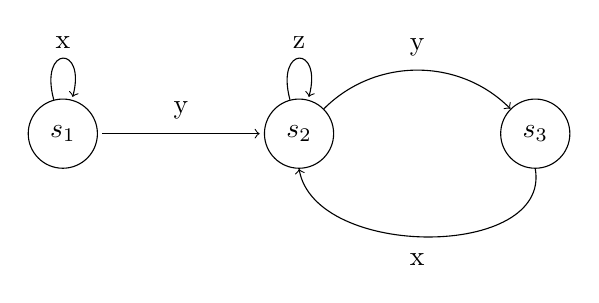
\begin{tikzpicture}
      \node[state] (q1) at (0,0) {$s_1$};
      \node[state] (q2) at (3,0) {$s_2$};
      \node[state] (q3) at (6,0) {$s_3$};
      \draw (q1) edge[loop above] node{x} (q1)
      (q2) edge[loop above] node{z} (q2);
      \draw[->] (q2) to [out=45] (q3);
      \draw[->] (q3.south) to [out=280,in=280] (q2.south);
      \draw[->](0.5,0)--(2.5,0);
      \node[fill=white] at (1.5,0.3) {y};
      \node[fill=white] at (4.5,1.1) {y};
      \node[fill=white] at (4.5,-1.6){x};
    \end{tikzpicture}
  \end{center}
\end{frame}
\section{Prove: Finite automaton accept rational languages}
\section{Prove: Every rational language is accepted by a finite automaton}
\section{Overview Weighted Automatons}
\section{Conclusion}




\begin{frame}
    \Huge{\centerline{Thanks for your attention!}}
    % \Huge{\centerline{Any Questions?}}
    
\end{frame}



\bibliography{references}
\bibliographystyle{acl_natbib}
\end{document}
